\documentclass[11pt,a4paper]{article}

\usepackage[utf8]{inputenc}
\usepackage[margin=0.5in]{geometry}
\usepackage{xcolor}
\usepackage{tikz}
\usetikzlibrary{arrows.meta, calc}

\pagestyle{empty} % Standalone single page

% Styles for Clean, High-Contrast Black & White Architecture
\tikzset{
    tierframe/.style={
        draw=black,
        fill=white,
        line width=1.1pt,
        rounded corners=5pt
    },
    compbox/.style={
        draw=black!75,
        fill=white,
        line width=0.7pt,
        rounded corners=3pt,
        font=\footnotesize\sffamily,
        text=black,
        align=center,
        inner sep=5pt
    },
    flowarrow/.style={
        -{Stealth[length=6pt, width=4.5pt]},
        thick,
        draw=black
    },
    dasharrow/.style={
        -{Stealth[length=6pt, width=4.5pt]},
        dashed,
        thick,
        draw=black
    }
}

\begin{document}

\begin{center}
    {\LARGE \textbf{ Architecture Diagram : Python Lists in C++}}\\[0.3em]
   
\end{center}

\vspace{0.4em}

\begin{figure}[htbp]
\centering
\resizebox{\textwidth}{!}{
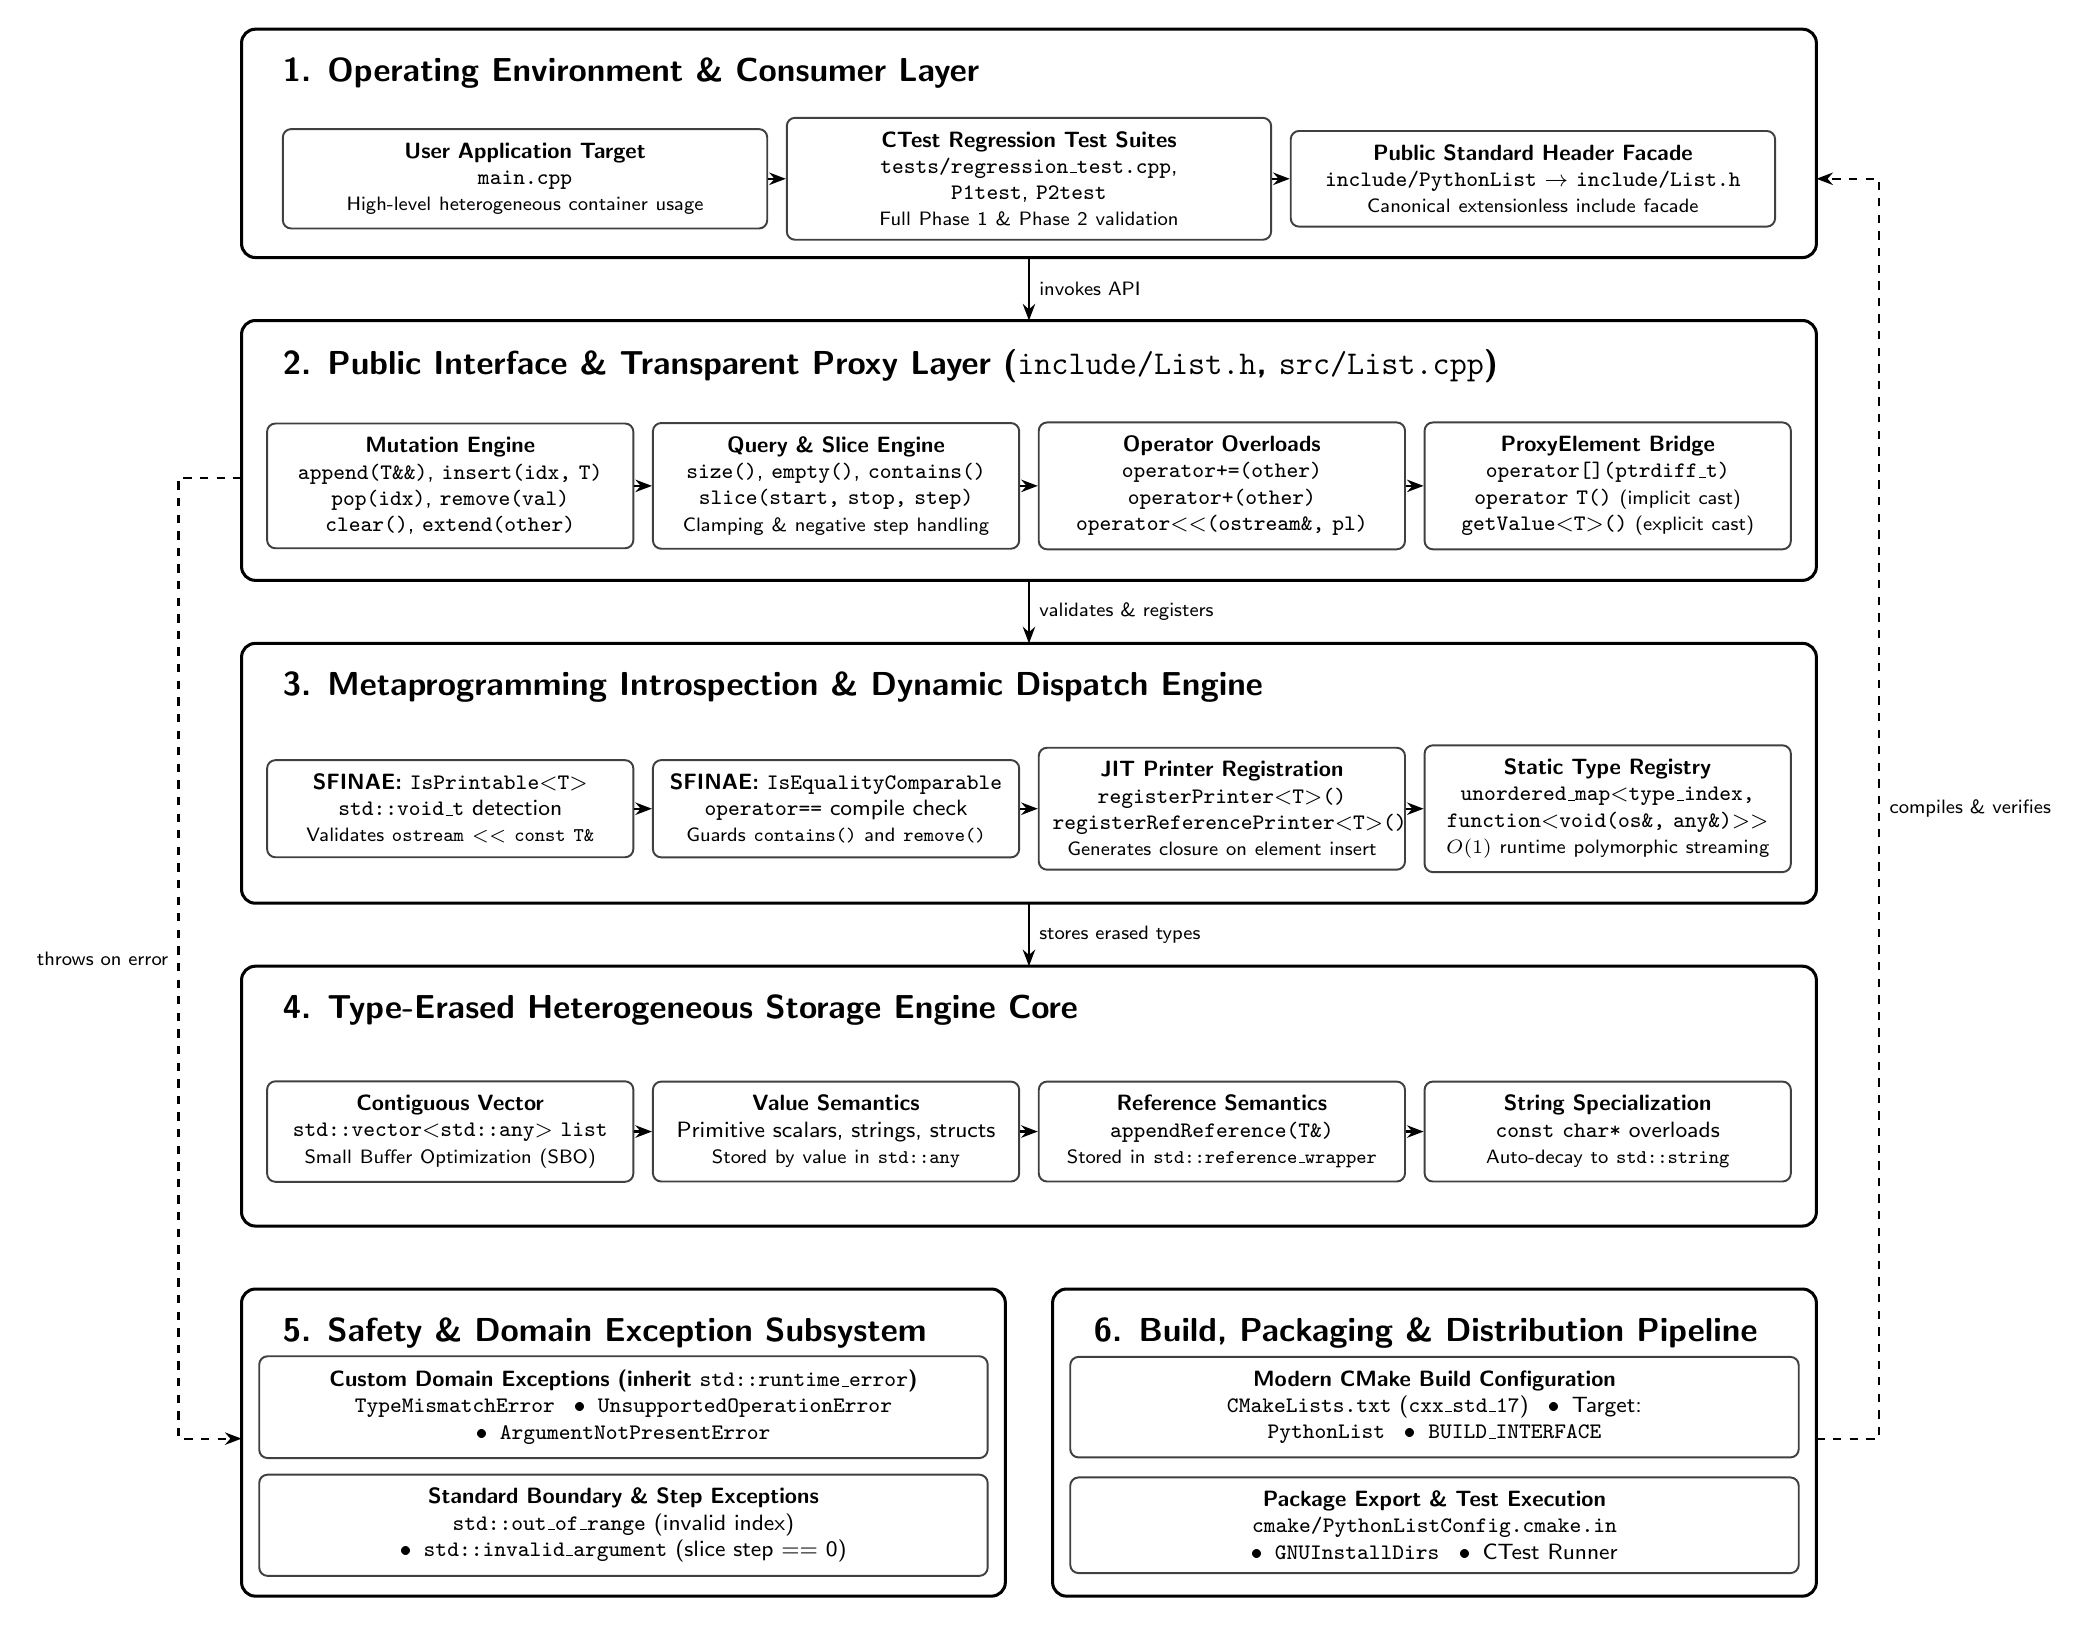
\begin{tikzpicture}

    % =========================================================================
    % TIER 1: CLIENT & OPERATING ENVIRONMENT
    % =========================================================================
    \draw [tierframe] (-10.0, 7.8) rectangle (10.0, 10.7);
    \node [anchor=north west, font=\large\bfseries\sffamily, text=black] at (-9.6, 10.45) 
          {1. Operating Environment \& Consumer Layer};

    \node (app) [compbox, text width=5.8cm] at (-6.4, 8.8) {
        \textbf{User Application Target}\\
        \texttt{main.cpp}\\
        {\scriptsize High-level heterogeneous container usage}
    };

    \node (tests) [compbox, text width=5.8cm] at (0.0, 8.8) {
        \textbf{CTest Regression Test Suites}\\
        \texttt{tests/regression\_test.cpp}, \texttt{P1test}, \texttt{P2test}\\
        {\scriptsize Full Phase 1 \& Phase 2 validation}
    };

    \node (wrapper) [compbox, text width=5.8cm] at (6.4, 8.8) {
        \textbf{Public Standard Header Facade}\\
        \texttt{include/PythonList} $\rightarrow$ \texttt{include/List.h}\\
        {\scriptsize Canonical extensionless include facade}
    };

    \draw [flowarrow] (app.east) -- (tests.west);
    \draw [flowarrow] (tests.east) -- (wrapper.west);

    % =========================================================================
    % TIER 2: PUBLIC INTERFACE & PROXY TIER
    % =========================================================================
    \draw [tierframe] (-10.0, 3.7) rectangle (10.0, 7.0);
    \node [anchor=north west, font=\large\bfseries\sffamily, text=black] at (-9.6, 6.75) 
          {2. Public Interface \& Transparent Proxy Layer (\texttt{include/List.h}, \texttt{src/List.cpp})};

    \node (mutators) [compbox, text width=4.3cm] at (-7.35, 4.9) {
        \textbf{Mutation Engine}\\
        \texttt{append(T\&\&)}, \texttt{insert(idx, T)}\\
        \texttt{pop(idx)}, \texttt{remove(val)}\\
        \texttt{clear()}, \texttt{extend(other)}
    };

    \node (queries) [compbox, text width=4.3cm] at (-2.45, 4.9) {
        \textbf{Query \& Slice Engine}\\
        \texttt{size()}, \texttt{empty()}, \texttt{contains()}\\
        \texttt{slice(start, stop, step)}\\
        {\scriptsize Clamping \& negative step handling}
    };

    \node (operators) [compbox, text width=4.3cm] at (2.45, 4.9) {
        \textbf{Operator Overloads}\\
        \texttt{operator+=(other)}\\
        \texttt{operator+(other)}\\
        \texttt{operator\textless\textless(ostream\&, pl)}
    };

    \node (proxy) [compbox, text width=4.3cm] at (7.35, 4.9) {
        \textbf{ProxyElement Bridge}\\
        \texttt{operator[](ptrdiff\_t)}\\
        \texttt{operator T()} {\scriptsize (implicit cast)}\\
        \texttt{getValue\textless T\textgreater()} {\scriptsize (explicit cast)}
    };

    \draw [flowarrow] (mutators.east) -- (queries.west);
    \draw [flowarrow] (queries.east) -- (operators.west);
    \draw [flowarrow] (operators.east) -- (proxy.west);

    % =========================================================================
    % TIER 3: METAPROGRAMMING & DYNAMIC DISPATCH ENGINE
    % =========================================================================
    \draw [tierframe] (-10.0, -0.4) rectangle (10.0, 2.9);
    \node [anchor=north west, font=\large\bfseries\sffamily, text=black] at (-9.6, 2.65) 
          {3. Metaprogramming Introspection \& Dynamic Dispatch Engine};

    \node (sfinae_print) [compbox, text width=4.3cm] at (-7.35, 0.8) {
        \textbf{SFINAE: \texttt{IsPrintable\textless T\textgreater}}\\
        \texttt{std::void\_t} detection\\
        {\scriptsize Validates \texttt{ostream \textless\textless\ const T\&}}
    };

    \node (sfinae_eq) [compbox, text width=4.3cm] at (-2.45, 0.8) {
        \textbf{SFINAE: \texttt{IsEqualityComparable}}\\
        \texttt{operator==} compile check\\
        {\scriptsize Guards \texttt{contains()} and \texttt{remove()}}
    };

    \node (jit_printer) [compbox, text width=4.3cm] at (2.45, 0.8) {
        \textbf{JIT Printer Registration}\\
        \texttt{registerPrinter\textless T\textgreater()}\\
        \texttt{registerReferencePrinter\textless T\textgreater()}\\
        {\scriptsize Generates closure on element insert}
    };

    \node (printer_map) [compbox, text width=4.3cm] at (7.35, 0.8) {
        \textbf{Static Type Registry}\\
        \texttt{unordered\_map\textless type\_index,}\\
        \texttt{function\textless void(os\&, any\&)\textgreater\textgreater}\\
        {\scriptsize $O(1)$ runtime polymorphic streaming}
    };

    \draw [dasharrow] (sfinae_print.east) -- (sfinae_eq.west);
    \draw [flowarrow] (sfinae_eq.east) -- (jit_printer.west);
    \draw [flowarrow] (jit_printer.east) -- (printer_map.west);

    % =========================================================================
    % TIER 4: HETEROGENEOUS STORAGE CORE
    % =========================================================================
    \draw [tierframe] (-10.0, -4.5) rectangle (10.0, -1.2);
    \node [anchor=north west, font=\large\bfseries\sffamily, text=black] at (-9.6, -1.45) 
          {4. Type-Erased Heterogeneous Storage Engine Core};

    \node (vec_storage) [compbox, text width=4.3cm] at (-7.35, -3.3) {
        \textbf{Contiguous Vector}\\
        \texttt{std::vector\textless std::any\textgreater\ list}\\
        {\scriptsize Small Buffer Optimization (SBO)}
    };

    \node (val_semantics) [compbox, text width=4.3cm] at (-2.45, -3.3) {
        \textbf{Value Semantics}\\
        Primitive scalars, strings, structs\\
        {\scriptsize Stored by value in \texttt{std::any}}
    };

    \node (ref_semantics) [compbox, text width=4.3cm] at (2.45, -3.3) {
        \textbf{Reference Semantics}\\
        \texttt{appendReference(T\&)}\\
        {\scriptsize Stored in \texttt{std::reference\_wrapper}}
    };

    \node (cstring_decay) [compbox, text width=4.3cm] at (7.35, -3.3) {
        \textbf{String Specialization}\\
        \texttt{const char*} overloads\\
        {\scriptsize Auto-decay to \texttt{std::string}}
    };

    \draw [flowarrow] (vec_storage.east) -- (val_semantics.west);
    \draw [flowarrow] (val_semantics.east) -- (ref_semantics.west);
    \draw [flowarrow] (ref_semantics.east) -- (cstring_decay.west);

    % =========================================================================
    % TIER 5: SAFETY SUBSYSTEM (BOTTOM LEFT)
    % =========================================================================
    \draw [tierframe] (-10.0, -9.2) rectangle (-0.3, -5.3);
    \node [anchor=north west, font=\large\bfseries\sffamily, text=black] at (-9.6, -5.55) 
          {5. Safety \& Domain Exception Subsystem};

    \node (custom_err) [compbox, text width=8.9cm] at (-5.15, -6.8) {
        \textbf{Custom Domain Exceptions (inherit \texttt{std::runtime\_error})}\\
        \texttt{TypeMismatchError} \enspace\textbullet\enspace
        \texttt{UnsupportedOperationError} \enspace\textbullet\enspace
        \texttt{ArgumentNotPresentError}
    };

    \node (std_err) [compbox, text width=8.9cm] at (-5.15, -8.3) {
        \textbf{Standard Boundary \& Step Exceptions}\\
        \texttt{std::out\_of\_range} (invalid index) \enspace\textbullet\enspace
        \texttt{std::invalid\_argument} (slice step == 0)
    };

    % =========================================================================
    % TIER 6: BUILD & DISTRIBUTION (BOTTOM RIGHT)
    % =========================================================================
    \draw [tierframe] (0.3, -9.2) rectangle (10.0, -5.3);
    \node [anchor=north west, font=\large\bfseries\sffamily, text=black] at (0.7, -5.55) 
          {6. Build, Packaging \& Distribution Pipeline};

    \node (cmake_box) [compbox, text width=8.9cm] at (5.15, -6.8) {
        \textbf{Modern CMake Build Configuration}\\
        \texttt{CMakeLists.txt} (\texttt{cxx\_std\_17}) \enspace\textbullet\enspace
        Target: \texttt{PythonList} \enspace\textbullet\enspace
        \texttt{BUILD\_INTERFACE}
    };

    \node (pkg_box) [compbox, text width=8.9cm] at (5.15, -8.3) {
        \textbf{Package Export \& Test Execution}\\
        \texttt{cmake/PythonListConfig.cmake.in} \enspace\textbullet\enspace
        \texttt{GNUInstallDirs} \enspace\textbullet\enspace
        CTest Runner
    };

    % =========================================================================
    % VERTICAL PIPELINE ARROWS (CENTER CHANNEL - ZERO OVERLAPS)
    % =========================================================================
    \draw [flowarrow] (0, 7.8) -- node[right, font=\scriptsize\sffamily, text=black] {invokes API} (0, 7.0);
    \draw [flowarrow] (0, 3.7) -- node[right, font=\scriptsize\sffamily, text=black] {validates \& registers} (0, 2.9);
    \draw [flowarrow] (0, -0.4) -- node[right, font=\scriptsize\sffamily, text=black] {stores erased types} (0, -1.2);

    % =========================================================================
    % OUTER PERIMETER CONNECTORS (STRICTLY OUTSIDE ALL BOXES - ZERO OVERLAPS)
    % =========================================================================
    % Outer left connector: Tier 2 -> Tier 5 (Throws on error)
    \draw [dasharrow] (-10.0, 5.0) -- ++(-0.8, 0) |- 
          node[pos=0.25, left, font=\scriptsize\sffamily, text=black] {throws on error} (-10.0, -7.2);

    % Outer right connector: Tier 6 -> Tier 1 (Compiles and tests)
    \draw [dasharrow] (10.0, -7.2) -- ++(0.8, 0) |- 
          node[pos=0.25, right, font=\scriptsize\sffamily, text=black] {compiles \& verifies} (10.0, 8.8);

\end{tikzpicture}
}
\end{figure}

\vspace{-0.2em}



\end{document}